\documentclass{ML}
\usepackage{amssymb}
\usepackage{latexsym}
% 姓名,学号
\infoauthor{朱明彦}{1160300314}

% 课程类型,实验名称
\infoexp{课程类型}{概述}

\infoschool{计算机学院}{高宏}

\begin{document}
\maketitle

\tableofcontents
\newpage

\begin{center}
    \textbf{\zihao{3} 论文概述}
\end{center}

\section{解决的问题}
选择的论文\cite{toain}为2018年PVLDB上面的一篇文章,\textbf{主要解决的问题是Road Networks上面动态的kNN查询}。

针对这个问题,作者主要有如下\textbf{三个方面}的工作:
\begin{enumerate}
    \item 对于Road Networks上需要进行kNN查询的系统建立新的数学模型,并找到其中影响系统整体吞吐量的关键因素。
    \item 建立了一个以Shortcut Graph为基础的索引,SCOB。
    \item 设计了可以根据Update/Query的所用时间动态调整SCOB以最大化系统吞吐量的算法,TOAIN。
\end{enumerate}
\section{采用的思想}
作者为了解决Road Networks上面动态的kNN查询,采用的思想是\textbf{先明确系统的目标(最大化系统的吞吐量),建立数学模型衡量寻找影响体统吞吐量的关键因素,对于关键的因素建立索引并利用设计的算法尽量提高关键因素影响下的部分,最终实现最大化吞吐量的目的}。

\begin{figure}[htb]
	\centering
	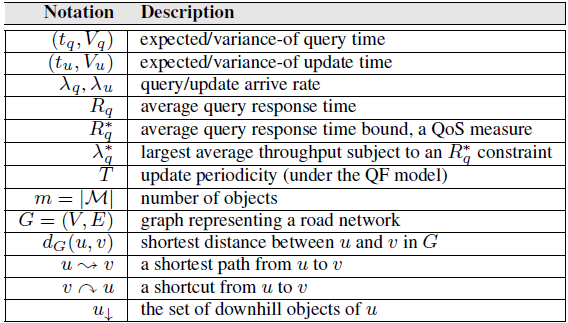
\includegraphics[width=0.8\linewidth]{media/notations.png}
	\caption{Notations}\label{fig:notations}
\end{figure}
\subsection{数学模型方面}
作者主要考虑了两种不同的情况,分别对应于现实中两种不同的应用,即\textbf{如滴滴类似的打车软件系统和捕捉精灵球的Pokemon}。 作者在考虑数学模型时,从\textbf{Query}和\textbf{Update}分别考虑其影响,然后针对这两种不同的应用区分它们在Query和Update上面的差别,从而建立起来不同的数学模型。

\textbf{以下两种应用都假设所有的查询到来是随机的,论文中为了方便假设Query符合泊松过程(Poisson Process)。}
\subsubsection{打车软件(BUA+QF Model)}\label{sec:bua_qf}
\textbf{BUA(Batch Update Arrival)模型是针对Update操作来说},其假设所有的元素都会进行Update操作,且都是在时间片的开始时刻进行,如果在某一个时间片里没有完成相应的Update操作,则直接舍弃未做操作,进行下一轮操作即可。\textbf{QF(Query First)是针对系统中队列模型来说的},其假设Query在队列中的优先级高于Update。

基于上面的假设,在打车软件这样的系统中,对于每个Query是来自用户的,查询在其附近最近的K个车辆;每个Update是来自汽车的,其在指定间隔内向系统返回其最新的位置。这样,高优先级的Query可以尽量减少用户请求的查询的延迟,并且丢失少量Update使得某些车辆的信息具有很短距离的差距,所以这样的假设对于该应用是合理的。

利用在\cite{single-server-queue}中的结论,可以得到式\eqref{equ:1},其中$R_q$为平均查询响应时间,$t_q, V_{q}$分别是查询时间的期望和方差,$\lambda_{q}$为Query到达的速率,即泊松过程中的参数。
\begin{equation}
R_{q}=\frac{\lambda_{q}\left(t_{q}^{2}+V_{q}\right)}{2\left(1-\lambda_{q^{t} q}\right)}+t_{q}
\label{equ:1}
\end{equation}

通过式\eqref{equ:1}可以看到,\textbf{整体的查询响应时间随$\lambda_{q}$的增大而增大,这也与我们的直觉相符合,说明此模型具有一定的道理}。进而通过两个约束,\textbf{查询的响应时间不能超过用户能够忍受的最大值}和\textbf{在一个时间间隔内需要最少的用于Update的时间限制},得到最终的$\lambda_{q}$的上界,如式\eqref{eq:2}所示。

\begin{equation}
\lambda_{q}^{*} \leq \min \left\{\frac{2\left(R_{q}^{*}-t_{q}\right)}{V_{q}+2 R_{q}^{*} t_{q}-t_{q}^{2}}, \quad\left(T-m t_{u}\right) /\left(T \cdot t_{q}\right)\right\}
\label{eq:2}
\end{equation}

为了可解释性,将式\eqref{eq:2}转化为式\eqref{eq:3}。
\begin{equation}
\lambda_{q}^{*} \leq \left\{
\begin{array}{lll}
{1 / t_{q},} & {\text { if } \alpha \beta<1 / 2} & {(\text { QoS-bound mode })} \\ 
{(1-\beta) / t_{q},} & {\text { if } \alpha \beta \geq 1 / 2} &\text {(Update-bound mode)}
\end{array}
\right.
\label{eq:3}
\end{equation}

其中$\alpha=R_{q}^{*} / t_{q} ; \quad \beta=m t_{u} / T ; \quad \gamma=V_{q} / t_{q}^{2}$;$\alpha$用来衡量平均查询相应时间的上界与平均查询时间的比值,$\beta$用来衡量一个时间片内处理Update所用时间的占比,$\gamma$是离散系数(coefficient of variation)的平方,相对于标准差其为无量纲量可以用在不同的索引算法中进行比较,一般$\gamma \in [0.1, 0.9]$。	

\subsubsection{Pokemon游戏(RUA+FCFS模型)}
对于pokemon类似的以所在位置为中心,查询周围存在的Pokemon,并进行捕捉的这类游戏,其Update不是按照某一指定的时间间隔返回的,而是随机的,所以其Update操作不能在使用BUA模型,而是转为RUA(Random Update Arrival)模型,同样的为了方便研究,\textbf{作者假设RUA的Update符合另一个泊松过程(与Query到来的泊松过程不同)}。

对于Query的优先级,Pokemon游戏很注重每个Pokemon的位置更新,所以该模型的队列模型使用了FCFS(First-come-first-served),即Query和Update具有相同的优先级,根据到来的顺序来进行操作。

其分析过程与\ref{sec:bua_qf}节类似,最终得到式\eqref{eq:rua_fcfs},衡量在该模型下的Query到来频率的上界。

\begin{equation}
\lambda_{q}^{*} \leq \min \left\{\frac{2\left(R_{q}^{*}-t_{q}\right)\left(1-\lambda_{u} t_{u}\right)-\lambda_{u}\left(V_{u}+t_{u}^{2}\right)}{V_{q}+2 R_{q}^{*} t_{q}-t_{q}^{2}}, \frac{1-\lambda_{\mathrm{u}} t_{u}}{t_{q}}\right\}
\label{eq:rua_fcfs}
\end{equation}

\subsection{索引SCOB方面}

\subsubsection{假设条件}\label{sec:assumptions}
在索引和算法方面,作者做出了两个假设,分别是:
\begin{enumerate}
	\item 抽象后的图G是无向图
	\item 所有节点的Rank是不一样的
\end{enumerate}

%这两个假设虽然在后面进行了放松,但本质上论文作者最终解决的问题也没有彻底摆脱这第一个假设的约束,这一部分在后面%TODO 
%详细来说。

\subsubsection{符号定义}
\paragraph{SHORTCUT SET $SC_{<}$}\label{para:shortcut_set} 给定一个图$G=(V, E)$和一个定义在$V \to \mathbb{N}$上的Rank Function,则一条捷径(shortcut)$u \curvearrowright v \in SC_{<}$当且仅当1.$u, v \in V$,2.$r(u) < r(v)$,3.对于从$u$到$v$上最短路上的中间任意节点$z$均有$r(z) < r(u)$。

从上面的定义我们可以直接得到一个结论,如式\eqref{lemma:3},其中$SC_{<}$是从$G$上导出的捷径图(shortcut graph),因为不一定所有的$G$上的最短路都符合$r(z) < r(u)$即上述定义的第3条规则。
\begin{equation}
d_{G}(u, v) \leq d_{SC_{<}}(u, v) \quad \forall u, v \in V
\label{lemma:3}
\end{equation}
\paragraph{SUMMIT NODE}
给定一个最短路径(shortest path)$s \leadsto t$,则对于该最短路的Summit Node是$s \leadsto t$上具有最高权重的节点。

根据$SC_{<}$和summit node的定义以及第一个假设,我们可以直接得到式\eqref{lemma:4},其中$x$是最短路径$s \leadsto t$上的summit node。
\begin{equation}
d_{G}(s, t)=d_{SC_{<}}(s, x)+d_{SC_{<}}(t, x)
\label{lemma:4}
\end{equation}
\paragraph{DOWNHILL OBJECTS}
论文中作者为了形象表示不同节点的rank不同,具有越高rank的节点在图中的位置越高,如图\ref{fig:downhill}所示。基于这种形象的表示,如果在$SC_{<}$中有一条从$v$指向$u$的shortcut,则称$v$是$u$的downhill object。
\begin{figure}[htb]
	\centering
	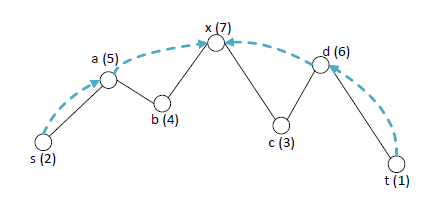
\includegraphics[width=0.6\linewidth]{media/downhill.png}
	\caption{Downhill Objects Example}\label{fig:downhill}
\end{figure}
\paragraph{$\mathbf{kDNNs}$}
给定一个节点$u \in G$,离它最近的k个downhill objects被记作$kDNN(u)$。

\subsubsection{基本思想}\label{sec:scob_basic}
根据式\eqref{lemma:3}和$G$是无向图的假设,可以有结论\textit{给定一个节点$s$和一个位于节点$t$的物体$o$,如果$o$是$s$的kNN之一,则有$o \in kDNN(x)$,$x$是最短路$s \leadsto t$上的summit node}(其证明使用了证明其逆否命题的方法,主要利用三角不等式、式\eqref{lemma:3}进行放缩)。\textbf{通过以上结论,可以利用kDNN和一些特定的summit node可以得到一些源点的KNN结果。}

SCOB索引本质上也是利用了Dijkstra在图上进行搜索,而传统的方式对于一个有M个节点的图,需要进行M次s-climb(从源点到summit node的搜索)以及M次t-climb(从目标点到summit node的搜索);而使用了SCOB索引\textbf{在每个summit node上记录在Shortcut Graph中的k个最近的downhill objects的id和其距离,以减少s-climb(t-climb)的次数,来提高效率,最终实现了仅需要从Query发出的节点进行一次s-climb就可以找到对应这次Query的kNN结果}。

具体如何维护SCOB索引,见\ref{sec:scob_index}节。

\subsubsection{假设条件放松}\label{sec:assumptions_release}
对\ref{sec:assumptions}节提到的两个假设,论文中分别进行了放松。对于第一个假设,其仅仅提到了一些做法,但在实际中可能并不适用,具体解释见\ref{sec:shortcoming}节。

对于第二个假设,作者修改了\ref{para:shortcut_set}节中shortcut的定义,其中第2点改为$r(u) \leq r(v)$,进而将如此导出的图记为$SC_{\leq}$。进而称在$SC_{<}$上的climb为straight climb,而在$SC_{\leq}$上的climb为gentle climb。
\subsection{算法TOAIN方面}
\subsubsection{符号定义}\label{sec:toain_def}
\paragraph{COVER NODES, COVER DIMENSION}
将Road Network放在二维空间上的地图,然后利用$K \times K$个方格将其分成$K^2$个cell,对于给定的cell $C$,其外面有$3 \ times 3$和$5 \times 5$的邻居,则对于处在$C$的节点$u$,如果$u \leadsto v$必须穿过$3 \times 3$的邻居,其中在最短路径上且跨过边界的边$(x, y)$,那么称$x$为$C$的一个Cover Node,所有这样的Cover Node的数量称为Cover Dimension。\textbf{例子见\ref{sec:example_cover_nodes}节说明}。

\subsubsection{基本思想}
TOAIN能够通过调整Rank function来调整SCOB索引的参数,寻找Query和Update之间的折中,进而达到最大化吞吐量的目的。所以\textbf{TOAIN的主要思想就是如何确定更合理的Rank Function,使得越重要的顶点具有越高的Rank}。具体的算法描述见\ref{sec:toain_compute_rank}节所示。
\section{基本算法描述}
文中以伪代码形式讲述的算法共有4个,下面将分别进行描述。
\subsection{SCOB Index}\label{sec:scob_index}
\subsubsection{Query}
\begin{figure}[htb]
	\centering
	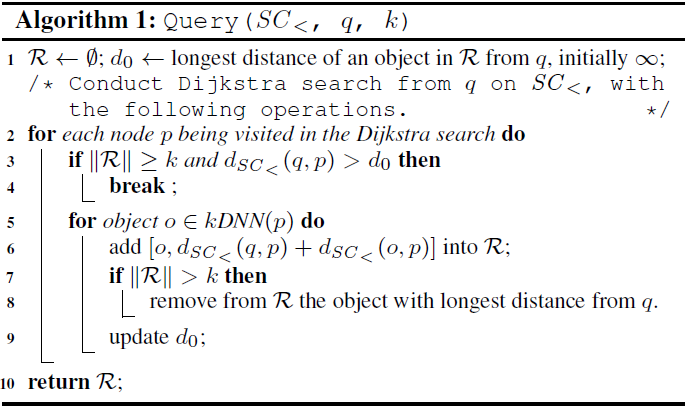
\includegraphics[width=0.6\linewidth]{media/query.png}
	\caption{Query Algorithm}\label{fig:query}
\end{figure}
在SCOB索引上进行kNN查询,主要是利用从查询所在的节点开始Dijkstra算法,对于每一个遇到的节点利用其kDNN更新最终的结果集合$\mathcal{R}$,直到遍历完所有节点或者$\mathcal{R}$中已有k个节点且当前遇到的节点在$SC_{<}$中的距离已经超过$\mathcal{R}$中的最大距离停止。算法如图\ref{fig:query}所示。

\textbf{由于其利用的是Dijkstra从原点进行搜索,所以其复杂度为$O(k|V|log|V|)$}。
\subsubsection{Insert}
\begin{figure}[htb]
	\centering
	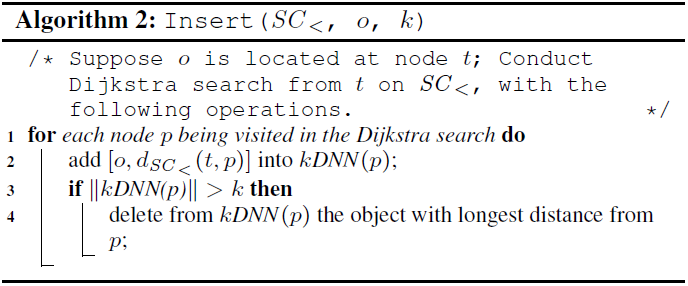
\includegraphics[width=0.6\linewidth]{media/insert.png}
	\caption{Insert Algorithm}\label{fig:insert}
\end{figure}
对于插入一个物体$o$,则进行从$o$所在节点$t$的Dijkstra算法,更新所有中间经过的节点的kDNN集合。算法如图\ref{fig:insert}所示。

\textbf{复杂度同样是Dijkstra的复杂度,即$O(|V|log|V|)$}。
\subsubsection{Delete}
\begin{figure}[htb]
	\centering
	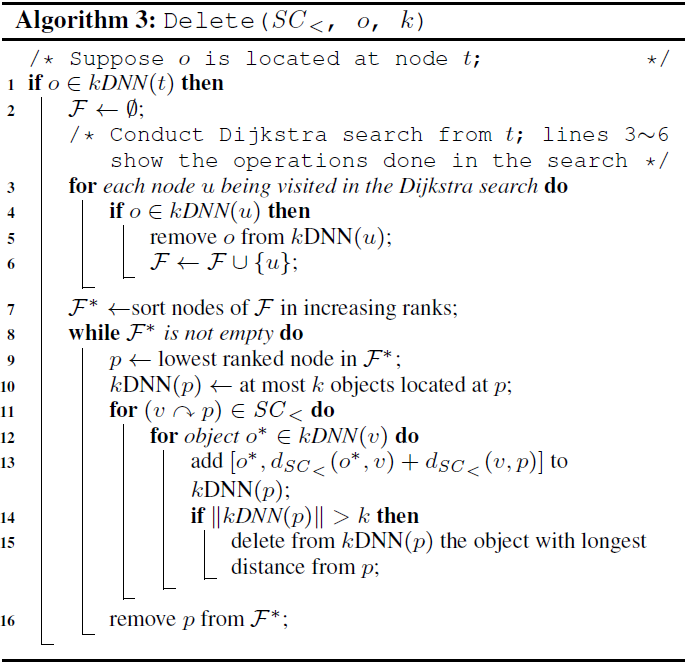
\includegraphics[width=0.6\linewidth]{media/delete.png}
	\caption{Delete Algorithm}\label{fig:delete}
\end{figure}
删除一个物体$o$,则需要首先判断该物体是否在其所在节点的kDNN集合中,如果不在算法直接结束;否则,需要从该顶点进行Dijkstra算法,对所有经过且kDNN包含物体$o$的节点,将$o$从其对应的kDNN集合中删除,并且对于所有上述节点补充新的物体进入kDNN集合。算法如图\ref{fig:delete}所示。

\textbf{复杂度为$O(|V|log|V| + |V||E|)$}。

\textbf{对于系统中涉及到的Update操作,没有直接给出相应的算法,而是改为用一次Insert和一次Delete操作进行代替。}
\subsection{TOAIN}\label{sec:toain_compute_rank}
\subsubsection{Compute Rank}
\begin{figure}[htb]
	\centering
	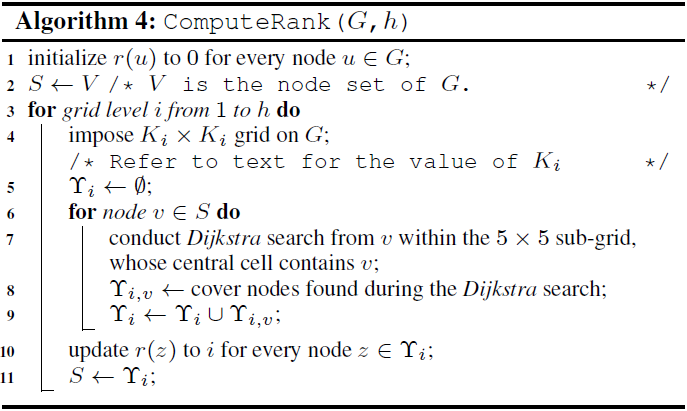
\includegraphics[width=0.6\linewidth]{media/compute_rank.png}
	\caption{Compute Rank Algorithm}\label{fig:compute_rank}
\end{figure}
根据\ref{sec:toain_def}节的定义,可以有结论\textbf{较大Cell对应的Cover Nodes具有较高的重要性,且较高重要性的Cover Nodes应具有较高的Rank}。

所以如图\ref{fig:compute_rank}所示的算法,先初始化所有的顶点rank为0,然后从1到h开始循环,较大的K逐步利用Dijkstra搜索进行更新遇到节点的rank值,同时不断减小K。

\textbf{由于每次K对半分,所以Dijkstra经过的节点数目不超过$O(\zeta^*)$(Cover Dimension的上限),所以整体的复杂度为$O(h\zeta^*|V|log|V|)$}

\subsubsection{climb}\label{sec:climb}
对于TOAIN下面的climb,每次所经过的节点不会超过$h\zeta^*$个,根据上一节的分析显然成立,所以进行一次climb的时间复杂度为$O(h\zeta^*)$。

\section{结论}
根据\ref{sec:scob_basic}节,文中提出的算法针对每一次Query仅需一次s-climb,而根据\ref{sec:climb}可知每次climb的复杂度不超过$O(h\zeta^*)$,每一次Query时间复杂度为$O(h\zeta^*)$。调整$h$可以调整Query和Update之间的时间,从而达到最大化吞吐量的目的。

根据\cite{zeta-most},$\zeta^*$不会很大,所以Computer Rank实际的复杂度接近$O(|V|log|V|)$。

最后根据论文中的实验结果,也侧面证实了其在相关算法中,无论对于实际例子还是生成数据,无论是BUA+QF模型还是RUA+FCFS模型,SCOB和TOAIN都是用时最少的。
\section{举例说明}
\subsection{COVER NODES, COVER DIMENSION}\label{sec:example_cover_nodes}
如图\ref{fig:cover_nodes}所示,对于给定的Cell $C$,位于其中的节点$u$,其$3\times3, 5 \times 5$的邻居均在图中标出。其中对于$u$与任何节点的最短路而言,其均需要通过$i, d, o$中的一个才可以到达,而$(u, d), (u, i), (u, o)$均跨过了$C$的边界,所以$i, d, o$均为Cover Nodes,且$C$的Cover Dimension为3。

\begin{figure}[htb]
	\centering
	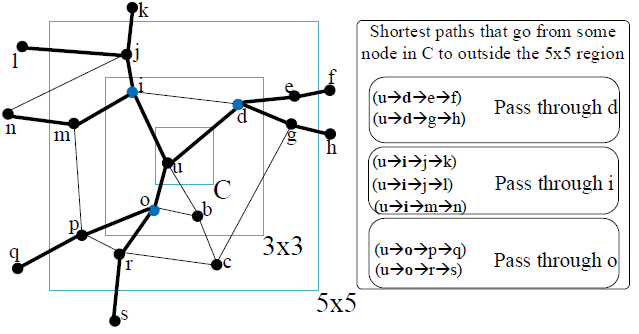
\includegraphics[width=0.7\linewidth]{media/cover_nodes.png}
	\caption{Cover Nodes example}\label{fig:cover_nodes}
\end{figure}

\subsection{COMPUTER RANK}
如图\ref{fig:example loop 1}所示,初始化$K=10$,$h=2$,图中所有的蓝色标记表示一个节点,红色数字表示该节点的rank值,橙色线段表示边,黑色方框表示Grid。
\begin{figure}[htb]
	\centering
	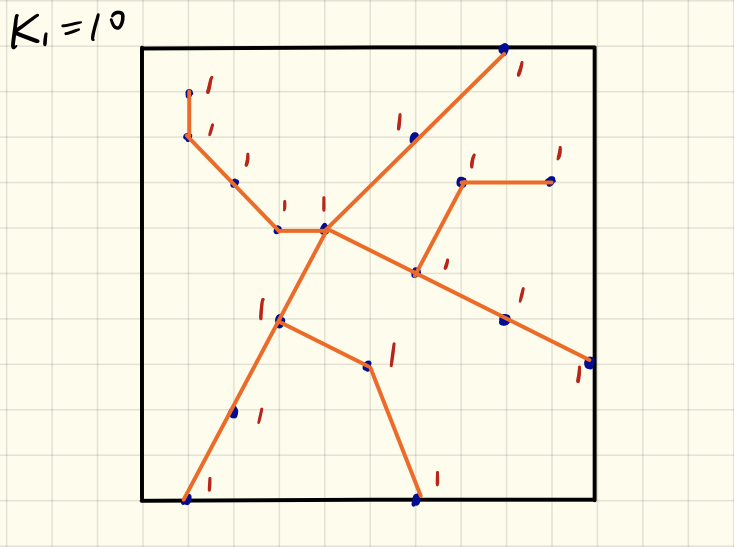
\includegraphics[width=0.7\linewidth]{media/example-1.jpg}
	\caption{Loop 1}\label{fig:example loop 1}
\end{figure}

\textbf{可以看到,在初始化的第一次循化会将所有节点的Rank都更新为1,此时的$S$仍然包含所有的节点。}

进入第二轮循环,此时$K$被更新为5,所有的Dijkstra算法都不会超过其对应的最小的$5 \times 5$的Grid。所有cover nodes的权值被更新为2,如图\ref{fig:example loop 2}所示。
\begin{figure}[htb]
	\centering
	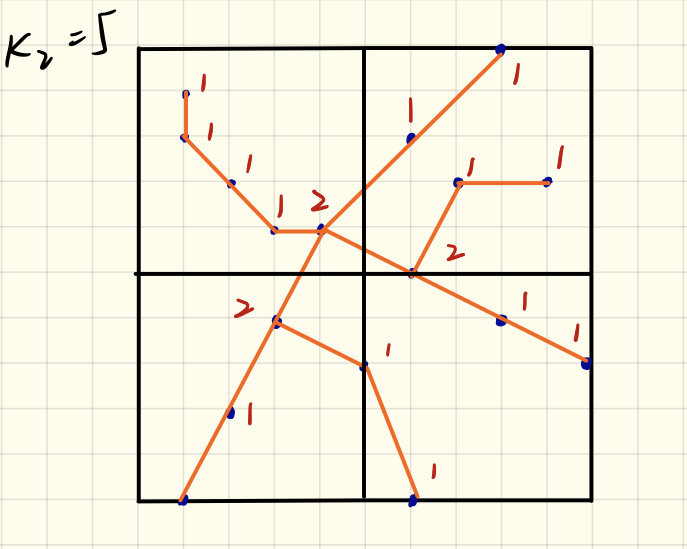
\includegraphics[width=0.7\linewidth]{media/example-2.jpg}
	\caption{Loop 2}\label{fig:example loop 2}
\end{figure}

由于继续更新,$K$会小于5,而此时与循环中需要对其所在的$5 \times 5$的Grid进行Dijkstra算法,所以$K$不够大导致算法停止,最终结果如图\ref{fig:example loop 2}所示。\textbf{可以看到,最终Rank值较大的节点,也是具有较高连通度的节点,这与使用\textit{betweenness centrality}进行rank赋值,具有相似性,说明了此算法的合理性}。
\section{算法的不足}\label{sec:shortcoming}
在论文中,作者提出放松\ref{sec:assumptions}节中第一个假设的方式,是针对将有向图的所有边均取反,这种做法可能导致整体计算Shortcut Graph时间复杂度变化,并且在现实中确实\textbf{存在单行线},如果简单对其取反可能缺少实际的物理意义,继而可能引入并不存在的边导致实际距离估计偏差较大的问题,如存在最短路径$s \leadsto t$,且$x$为其上的summit node,而此时$d_{SC_{<}}(t, x) \neq d_{SC_{<}}(x, t)$,进而导致式\eqref{lemma:4}不成立。

在相关的实验中,作者也没有进行关于Road Network中真正存在单向边,无法将其转化为无向图处理的情况提供相应的实验数据,也侧面说明了在这一部分TOAIN和SCOB结合起来对于存在大量单向边的情况处理有所困难。
\section{改进方法}

\section{相关工作}
使用Dijkstra算法进行kNN查询,从查询q所在的节点开始进行Dijkstra算法,直到有k个最近的物体被搜索到即可。

ROAD\cite{ROAD}同样是基于Dijkstra算法,但是主要是针对物体在network上面稀疏分布的情况。主要思想是将大图划分成若干个小图(文中称为Rnets),然后在利用Dijkstra搜索时如果某个小图(Rnet)中没有物体,则关于这个小图的搜索就被跳过。

G-Tree\cite{G-tree}也是建立了子图的层次结构,但是每个子图都与一个Occurrence-List关联,利用OL按照ID降序记录子图的层次结构。也因为其记录了更多的信息,所以在G树上查询很快,但更新较慢。

V树\cite{V-tree}采用与G树类似的层次结构。V树标识位于子图边界的边界节点。通过维护这些边界节点的最近对象列表,设计了有效的技术来回答kNN查询。

\appendix

% \section{源代码}
% \section{参考文献}
\begin{thebibliography}{20}
    \bibitem{toain} Luo, S., Kao, B., Li, G., Hu, J., Cheng, R., \& Zheng, Y. (2018). TOAIN: a throughput optimizing adaptive index for answering dynamic k NN queries on road networks. Proceedings of the VLDB Endowment, 11(5), 594-606.
    \bibitem{single-server-queue} J. W. Cohen. The single server queue, volume 8. Elsevier, 2012.
    \bibitem{zeta-most}S. Luo, R. Cheng, X. Xiao, B. Kao, S. Zhou, and J. Hu. Fast
    matching of detour routes and service areas. Technical
    Report TR-2016-03, The University of Hong Kong, 2016.
    \bibitem{ROAD}K. C. Lee, W.-C. Lee, B. Zheng, and Y. Tian. Road: A new
    spatial object search framework for road networks. TKDE,
    24(3):547–560, 2012.
    \bibitem{G-tree}R. Zhong, G. Li, K.-L. Tan, L. Zhou, and Z. Gong. G-tree:
    An efficient and scalable index for spatial search on road
    networks. TKDE, 27(8):2175–2189, 2015.
    \bibitem{V-tree}B. Shen, Y. Zhao, G. Li, Q. Y. Zheng, Weimin, B. Yuan, and
    Y. Rao. V-tree: Efficient knn search on moving objects with
    road-network constraints. In ICDE, pages 871–882, 2016.
\end{thebibliography}

\end{document}
